\chapter{Deep Learning}

An auspicious field of \acrlong{ml} is deep learning.

With the raise of graphic cards a concept from 1960 has become more interesting in recent years.

aims to overpower baseline approaches

\section{Splitting Data into different Sets}

A 

To avoid overfitting, a deep learning model should use at least two different training sets to 

\subsection{Test Set}

To make meaningful comparisons between different models, a standardised sample set needs to be used for validation. This data set consists of real-world examples or should at least simulate the planned use case as best as possible.

\subsection{Train, Test, and Validation Set}

we have 3 data sets used for deep learning

\begin{figure}[!ht]
    \centering
    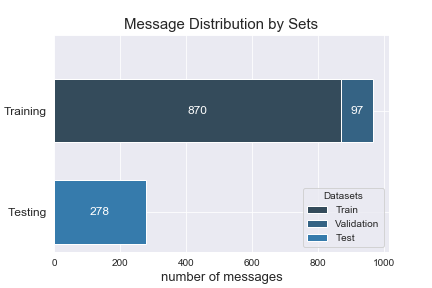
\includegraphics[scale=0.5]{plot-datasets}
    \caption{Different data sets}
    \label{fig:datasets}
\end{figure}

\section{Defining Input and Output Layers}

Write why the input is important and why the network can calculate the other dimensions according to the used layers itself.

\subsection{Sliding Windows}
\label{chap:sliding-window}

Due to different lengths of the text samples, the input layer of the neural network cannot rely on the number of words in the corpus. It has to be consistent throughout the whole training and validation process. One possible solution is to adjust the input dimension to the size of the longest sentence in the corpus, but this would wastefully bloat the network's parameter space. Needless to say that this enormous structure is only used by the longest text and is an overhead for all other input values. Another possibility is to use the \verb|pad_sequences()|\footnote{more information at https://keras.io/preprocessing/sequence} function of \emph{Keras} which simply trims sentences to a specific length. Unfortunately many tokens at the end of texts will get cut off.

A well-constructed deep learning model shouldn't only rely on a single token to make its predictions. Especially in \acrshort{nlp} the context is fundamental for making suitable predictions. Therefore the sliding window functionality comes in very handy. It creates multiple windows with of a defined length but with different tokens. Every token of a text is at least once present in a window. Listing \ref{code:sliding-window} shows how these slices are generated.

Table \ref{tbl:sliding-window} illustrates the \verb|sliding_window()| function with an example. The colourized cell indicates the current token which the network should predict. This single sentence results in eight windows. The sliding window technique duplicates the input data thus the original 967 sentences are split into 70354 windows of size 9.

\begin{table}[ht!]
    \centering
    \begin{tabular}{|c|c|c|c|c|c|c|c|c|}
        \hline
        \verb|i| & \multicolumn{7}{c|}{\textbf{Sliding Window}} \\ [0.5ex]
        \hline
        1 &  &  &  & \cellcolor[HTML]{eaeaf2} Bond & drinks & his & vodka \\ [0.5ex]
        \hline
        2 &  &  & Bond & \cellcolor[HTML]{eaeaf2} drinks & his & vodka & martini \\ [0.5ex]
        \hline
        3 &  & Bond & drinks & \cellcolor[HTML]{eaeaf2} his & vodka & martini & shaken, \\ [0.5ex]
        \hline
        4 & Bond & drinks & his & \cellcolor[HTML]{eaeaf2} vodka & martini & shaken, & not \\ [0.5ex]
        \hline
        5 & drinks & his & vodka & \cellcolor[HTML]{eaeaf2} martini & shaken, & not & stirred. \\ [0.5ex]
        \hline
        6 & his & vodka & martini & \cellcolor[HTML]{eaeaf2} shaken, & not & stirred. & \\ [0.5ex]
        \hline
        7 & vodka & martini & shaken, & \cellcolor[HTML]{eaeaf2} not & stirred. &  & \\ [0.5ex]
        \hline
        8 & martini & shaken, & not & \cellcolor[HTML]{eaeaf2} stirred. &  &  & \\ [0.5ex]
        \hline
    \end{tabular}
    \caption{Sliding windows of size 7}
    \label{tbl:sliding-window}
\end{table}

\subsection{Using Keras Tokenizer}

The input into a neural network has to be numeric. Therefore a very simple solution is to map every word to an unique ID. The \emph{Keras tokenizer} creates an ID for every distinctive word in the training data. As seen in table \ref{tbl:keras-tokenizer} the IDs are ranked by their frequency in the text. The words \emph{to} and \emph{be} are more frequent than the rest so they have got a lower ID.

\begin{table}[ht!]
    \centering
    \begin{tabular}{|l|c|c|c|c|c|c|c|c|c|c|}
        \hline
        \textbf{Original} & To & be, & or & not & to & be, & that & is & the & question. \\
        \hline
        \textbf{Tokenized} & 2 & 3 & 4 & 5 & 2 & 3 & 6 & 7 & 8 & 9 \\
        \hline
    \end{tabular}
    \caption{Example output of the Keras tokenizer}
    \label{tbl:keras-tokenizer}
\end{table}

The first ID is reserved for a special token called \emph{OOV} (out-of-vocabulary). You have to fit the tokenizer on a given text which may not contain the same tokens than the test set. Every word which the \emph{tokenizer} hasn't seen before gets labelled as \emph{OOV}. Consider listing \ref{code:keras-tokenizer} to see how the tokenizer is being used.

\subsubsection{Vocabulary}

Normally the tokenizer's vocabulary only consists of the tokens in the training set to emulate a real world scenario for the model. Because of language changes or misspelled words, unknown tokens aren't rare. Due to the sliding window technique, the input data gets multiplied by a factor of the exact window size. Therefore even a token which only occurs once in the whole data exists now several times. The \verb|train_test_split()| will most likely add at least one instance of this token to the train set. Multiple experiments confirm, that the tokenizer's word index contains more than 95\% of the vocabulary. It's a small flaw in the architecture, hence the model would perform slightly worse in production.

\subsubsection{Disadvantages}

The main downside of using a tokenizer is that the IDs doesn't provide any additional information about the token itself. For example the Swiss German word \emph{Velo}, which means bicycle, is probably more frequently used in the corpus than the German version \emph{Fahrrad}. These two words share a very strong similarity but this relation is invisible when using IDs. Another disadvantage is, that higher IDs might have higher weights than lower ones \cite{nurz18}. Therefore \emph{embeddings} should be used as described in section \ref{embeddings-chapter-here}.

\subsection{Output Layer}

To classify all tokens into the three classes \emph{O}, \emph{PER}, and \emph{LOC}, several solutions are applicable. Rather than getting a single neuron as output I chose to use three output neurons where all are representing a class. 

insert formula for softmax or sigmoid here

\section{Building the first Network}

\section{Enlarging the Network}

more units, more fun

\section{Implementing Class Weights}

\subsection{Calculate Weights with Scikit-learn}

\subsection{Set Weights out of the stomach}

\section{Using Embeddings}

\subsection{Create own Embeddings}

\subsection{Use Wikipedia Embeddings}

\section{Prevent from Overfitting with Dropout}

The dropouts are introduced in this paper \cite{drop14}
